\chapter{Virtual Network Embedding Problem}
\label{ch:problem}

As seem in Chapter~\ref{ch:relwork}, several variation of VNEP are presented in the literature. This work captures the essential components of the problem that make the problem hard to solve.

Virtual nodes consume resources from physical nodes. 
Generally CPU processing capacity and memory space are considered.
To simplify the modeling, just CPU processing is considered in this work.
Due to load balancing considerations \cite{Houidi:2011}, each virtual node has to be mapped to a different physical node.

Some applications have geographical restrictions due to the demand of connecting different geographical locations or security reasons \cite{Buriol:2012}.
Hence some formulations allow virtual nodes to be restricted to a subset of physical nodes.
As the formulation adopted in this work aims to be generic, no location constraints are considered.

Virtual links have to be mapped into physical paths between physical nodes that host their endpoints.
Multiple virtual links can share the same physical link.
A part of the limited bandwidth capacity of physical edges is reserved for each virtual link.

Finding a feasible link mapping is NP-Hard even if node mapping is fixed. In order to render the problem easier to solve, \citet{Yu2008} proposes a relaxation of the constraint that each virtual link has to be mapped into a single physical path.
By allowing virtual links to be mapped to multiple paths in the physical network, link mapping can be done in polynomial time.
Several works in the literature have taken this approach.
However, some applications, such as teleconferencing, do not allow the splitting of data \cite{Barnhart:2000} and 
current network technology do not generally support path splitting \cite{Guerzoni:2014}.
Therefore in this work path splitting is not allowed.

Other link mapping constraints found in the literature include routing capacities, delay limits, and limits on the sizes of paths \cite{infuhr:2011}.

All variations of VNEP aim for feasible mappings of virtual network nodes and links into physical resources. 
But different objective functions are considered such as minimizing the total cost of the mapping in networks where physical nodes and links have heterogeneous associated costs.
Others try to maximize the total profit when virtual networks have different revenues.
In this work, the objective function minimizes the amount of resources used by the obtained mapping.
Since all virtual nodes have to be mapped, a solution is evaluated by the used amount of bandwidth capacity of physical links.
Thus, for example, if a path with four links is used instead of one with two, the amount of bandwidth used is doubled.

Subsection~\ref{sec:def} presents a formal definition of the problem. It is followed by a presentation of the Integer Linear Models for VNEP in Subsection~\ref{sec:models}. The chapter ends with an analysis of the complexity of the problem in Subsection~\ref{sec:complexity}.

\section{Problem Definition}
\label{sec:def}

A VNEP instance has as input a virtual network and physical substrate network. The physical substrate is represented by an undirected graph $G^S = (V^S,E^S)$ with a CPU capacity of $C_{s}$ for each physical node $s \in V^S$ and a bandwidth capacity $B_{e}$ for each edge $e \in E^S$. The virtual network is represented by a undirected graph $G^V = (V^V,E^V)$ along with a demand $C_{v}$ for each virtual node $v \in V^V$, and a bandwidth demand of $B_{k}$ for each virtual link $k \in E^V$. 

The objective of the proposed problem is to find a feasible mapping of the virtual nodes and links onto the physical network with minimal cost. 
A feasible mapping is a pair of functions $(f_v, f_e)$: A mapping of nodes $f_v: V^V \rightarrow V^S$ and a mapping of links $f_{e=(w,u)}: E^V \rightarrow P$, where $P$ is the set of paths in the substrate graph with endpoints $f_v(w)$ and $f_v(u)$.
Each virtual node has to be mapped into a single substrate node with enough CPU capacity to host it. A substrate node can host at most one virtual node. Each virtual link $(w,u) \in E^V$ has to be mapped to a path in the physical graph between the nodes $f_v(w)$ and $f_v(u)$. An edge can host several virtual links, but the sum of their demands could not surpass the capacity of the edge. The cost of a mapping is the amount of bandwidth used in the physical network by the mapping.

Figure~\ref{fig:input} presents an instance of the problem composed of a physical network with four nodes and a virtual network with three nodes. 
Edges and nodes are labelled with their capacities or demands. 
%Next to each node label is the capacity or demand of the node.
The optimal mapping is shown in Figure~\ref{fig:mapping}. 
%Since the substrate node $d$ is the only one with enough capacity to host $p3$, 
The optimal solution is to map node $a$ to $C$, $b$ to $A$, and $c$ to $B$;
the virtual link  $(a,b)$ is mapped to $C-B-A$, and the virtual link $(b,c)$ is mapped to $A-B$. The cost of this solution is $50$.


%\tikzstyle{every node}=[draw, ellipse, minimum size=100pt,align=center]
\begin{figure}[!h]
  \centering
  \caption{An input instance for the VNEP.}\label{fig:input}   
  \begin{subfigure}[b]{0.45\linewidth}
  \centering    
  \subcaption{Physical Network}\label{fig:Physical}
\begin{tikzpicture}
\usetikzlibrary{arrows}
\usetikzlibrary{shapes}
\tikzstyle{every node}=[draw, ellipse, minimum size=10pt,align=center,scale=0.7]
\node at (0,0)(1){A (11)};
\node[below left=1cm of 1](2){B (16)};
\node[below right=1cm of 1](4){D (7)};
\node[below=2cm of 1](3){C (11)};
\path[every node/.style={font=\footnotesize},thick]
    (1) edge node[right] {10} (2)
	edge node[left] {30} (4)
    (2) edge node[right] {5} (3)
    (4) edge node[left] {30} (3);
\end{tikzpicture}
  \end{subfigure}  
  \begin{subfigure}[b]{0.53\linewidth}
  \centering
  \subcaption{Virtual Network}\label{fig:Virtual}
\begin{tikzpicture}
\usetikzlibrary{arrows}
\usetikzlibrary{shapes}
\tikzstyle{every node}=[draw, ellipse, fill=gray!40, minimum size=10pt, align=center, scale=0.7]
\node at (0,0)(1){a (10)};
\node[below=1cm of 1](2){b (10)};
\node[below=1cm of 2](3){c (15)};
\path[every node/.style={font=\footnotesize},thick]
    (1) edge[blue,densely dotted] node[right,color=black] {20} (2)
    (2) edge[red,thick,dashed] node[right,color=black] {10} (3);
\end{tikzpicture}
  \end{subfigure}   
\caption*{Source: from author (2015).}\end{figure}


\begin{figure}[!h]
  \centering
  \caption{Optimal solution for instance of Figure~\ref{fig:input}.\label{fig:mapping}}   
\begin{tikzpicture}
\usetikzlibrary{arrows}
\usetikzlibrary{shapes}
\tikzstyle{every node}=[draw, ellipse, minimum size=10pt,align=center,scale=0.7]
\node[fill=gray!40] at (0,0)(6){b(10)};
\node[below=0.5cm of 6] (1){A (11)};
\node[below left=1cm of 1](2){B (16)};
\node[below right=1cm of 1](4){D (7)};
\node[below=2cm of 1](3){C (11)};
\node[fill=gray!40, below=0.5cm of 1] (5){a(10)};
\node[fill=gray!40, above=0.5cm of 2] (7){c(15)};
\path[every node/.style={font=\footnotesize},thick]
    (5) edge[blue,densely dotted] node [] {} (3)
    (7) edge[red,dashed] node [] {} (2)
    (1) edge node [] {} (4)
    (2) edge[blue,densely dotted] node [] {} (3)
    (4) edge node [] {} (3);
  \draw[blue,thick,densely dotted] (2.25) -- (1.-135);
  \draw[red,thick,dashed] (2.40) -- (1.-150);
  \draw[blue,thick,densely dotted] (6.-80) -- (1.80);
  \draw[red,thick,dashed] (6.-100) -- (1.100);
\end{tikzpicture}
\caption*{Source: from author (2015).}\end{figure}

\section{Models}
\label{sec:models}
Most exact algorithms in the literature for the VNEP are based on ILP models. The following ILP model is based on~\cite{Alkmim2013}. It is adapted to the set of constraints presented in this work: let the decision variables $x_{v,s} = 1$ iff the substrate node $s$ hosts the virtual node $v$. And let $y_{v,w,s,j} = 1$ iff the physical link $(s,j)$ hosts the virtual link $(v,w)$.

\begin{align}
    \min & \sum\limits_{(s,j) \in E^{S}} \sum\limits_{(v,w) \in E^{V}} B_{v,w} y_{v,w,s,j} \label{eq:z} \\
    s.t. & \sum\limits_{v \in V^{V}} C_{v} x_{v,s} \leq C_{s}                     & \forall s \in V^{S}  \label{eq:flowcap} \\
    & \sum\limits_{s \in V^{S}} x_{v,s} = 1                                  & \forall v \in V^{V}  \label{eq:flowvirone}\\
         & \sum\limits_{v \in V^{V}} x_{v,s} \leq 1                               & \forall s \in V^{S} \label{eq:flowsubone}\\
         & \sum\limits_{j \in V^{S}} y_{v,w,s,j} - \sum\limits_{j \in V^{S}} y_{v,w,j,s} =  x_{v,s} - x_{w,s}  & \forall (v,w) \in E^{V}, s \in V^{S}\label{eq:flowflow} \\
         & \sum\limits_{(v,w) \in E^{V}} B_{v,w} y_{v,w,s,j} \leq B_{s,j}  & \forall (s,j) \in E^{S} \label{eq:flowbandwidth} \\
         & x_{v,s} \in \{0,1\} & \forall v \in V^{V}, s \in V^{S} \\
         & y_{k,l,m,n} \in \{0,1\} & \forall (k,l) \in E^{V}, (m,n) \in E^{S}
\end{align}

The objective function~\eqref{eq:z} minimizes the amount of bandwidth used by the virtual network. Constraints~\eqref{eq:flowcap} ensure that the capacities of substrate nodes are not surpassed. Constraints~\eqref{eq:flowvirone} and~\eqref{eq:flowsubone} enforce, respectively, that every virtual node is mapped to a different substrate node and every substrate node hosts at most one virtual node. Constraints~\eqref{eq:flowflow} are path constraints, they ensure that every virtual link is mapped to a path in the substrate graph. Finally, Equations~\eqref{eq:flowbandwidth} guarantee that the bandwidth capacities of physical edges are not violated.

Let us call this model \textbf{Compact Model} in contrast with the large model that will be presented later in this section.
As the VNEP is NP-Complete (a proof is given in Section~\ref{sec:complexity}), solving this ILP model is NP-Complete.
Branch \& Bound algorithms use linear relaxations to obtain bounds on optimal integer solutions.
The first problem with using the linear relaxation of the Compact Model is that there is no efficient algorithm to obtain integer solutions from that relaxation (proof in Section~\ref{sec:complexity}).
The second problem is that this relaxation provides a poor lower bound for the optimal solution, what has a negative impact on the performance of a Branch \& Bound algorithm.
It is always possible to obtain a solution with cost zero for the relaxation of this model.

\begin{proposition}
There is always a solution with cost zero to the compact model.
\end{proposition}

\begin{proof}
If every $x_{vs}$ is set to~$1 / |V^S| $, all constraints are respected and the left hand side of Constraints~\eqref{eq:flowflow} is zero. 
Therefore all variables $y_{vwsj}$ can be set to zero.
Hence, the cost of the optimal solution for the relaxed problem is always zero, resulting in a trivial lower bound.
\end{proof}
\vspace{-0.5cm}

\begin{comment}
Models based on Dantzig-Wolfe decomposition usually provide better lower bounds than compact models.
Also, the structure of the problem can be better exploited, resulting in a more efficient exploration of the solution space.

The Compact Model has a $p$-block angular structure, i.e., the model can be decomposed into $p$ independent blocks and $p$ linking blocks.
A $p$-block angular structure is illustrated in Figure~\ref{eq:pblock}.
Constraints~\eqref{eq:flowflow} present this kind of structure: each virtual link is independent of the other virtual links in those constraints and they are linked by Constraints~\eqref{eq:flowbandwidth}.
Thus, the problem can be decomposed in $|E^V|$ independent problems.
Each problem corresponds to a single virtual link mapping problem.

\begin{equation}
A = \left[  \begin{array}{cccc}
            A_{1} & A_{2} & \ldots & A_{p} \\
            B_{1} &       &        &       \\
                  & B_{2} &        &       \\
                  &       & \ddots &       \\
                  &       &        & B_{p} \\
            \end{array} \right] \label{eq:pblock}
\end{equation}

The polyhedron defined by the compact model is bounded, since all variables are binary, and it is nonempty (a two-phase method is used to guarantee that there is always a solution, c.f. Chapter~\ref{ch:cg}).
A nonempty and bounded convex polyhedron can be represented by a convex combination of its extreme points \cite{lasdon1970}.
Thus, let $C$ be the polyhedron defined by the Compact Model, any element $y \in C$ can be represented as:

\begin{align}
  y = & \sum\limits_{ j } \lambda_{j} x^{j} & \\
  where   & \sum\limits_{j} \lambda_{j} = 1 & \\
          & \lambda_{j} \geq 0              &
\end{align}

Where the $x^{j}$ are all the extreme points of polyhedron $C$.

Therefore, using Dantzig-Wolfe decomposition, we can reformulate the Compact Model as follows: Choose, from all valid paths, those that minimize the objective function. We follow to define a model based in paths that cover virtual links.

\begin{definition}
A substrate path $p = w_{1}, w_{2},\ldots, w_{n}$ ($w_{i} \in V^S, \forall i \in [n]$) \textbf{covers} the virtual link~$(u,v)$ if every edge in the path has enough capacity to host the virtual link, the first node $w_{1}$ in the path has enough CPU capacity to host virtual node $u$, and the last node $w_{n}$ has enough capacity to host the virtual node $w$.
\end{definition}

Let $P^k$ be the set of all paths in the physical network that cover the virtual link $k$.
We can write every $y_{k}$ as a convex combination of extreme points~$\{\delta_p\}_{p \in P^k}$.

\begin{align}
  y_{k} = & \sum\limits_{p \in P^{k}} \delta_{p} z_{p} \label{eq:yk} & \\
        %& x_{v,s} = \sum\limits_{(v,w) \in E^V} \sum\limits_{p \in P^{(v,w)}} \delta_{v,s,p} z_{p}
          & \sum\limits_{p \in P^k} z_{p} = 1 & \forall k \in E^V \\
          & z_{p} \in \{0,1\}                       & \forall k \in E^V, p \in P^k
\end{align}

%\begin{align}
%  s.t.  & \sum\limits_{p \in P^{k}} z_{p} = 1, z_{p} \geq 0 
%\end{align}

Therefore, each variable $y_{v,w,s,j}$ is uniquely defined in terms of paths in the graph as follows:

\begin{equation}
  y_{v,w,s,j} = \sum\limits_{p \in P^{(v,w)}} \delta_{s,j,p} z_{p} \label{eq:definition}
\end{equation}

Where $\delta_{s,j,p}$ is set to one iff the path $p$ contains the physical edge $(s,j)$.

If we replace the variables $y_{v,w,s,j}$ with variables $z_{p}$ in Constraints~\ref{eq:flowflow}:

\begin{align}
  \sum\limits_{j \in V^{S}} \sum\limits_{p \in P^k} \delta_{s,j,p} z_{p} - \sum\limits_{j \in V^{S}}\sum\limits_{p \in P^k} \delta_{j,s,p} z_{p} = x_{v,s} - x_{w,s}     & \quad \forall (v,w) = k \in E^{V}, s \in V^{S} \label{eq:flowwithpathvar}
\end{align}

Let $p = v_{1},v_{2},\ldots,v_{n}$ be a path in the substrate graph. Since $p$
is an undirected path in a graph, with exception of $j = v_{1}$ and $ j = v_{n}$,
the right hand side of the above equation is equal 
to zero. So this equation is equivalent to:

\begin{align}
  \sum\limits_{p \in P^k : (v,s) \in p} z_{p}
    - \sum\limits_{p \in P^k : (s,w) \in p} z_{p} 
    = x_{v,s} - x_{w,s}   
    & \quad \forall (v,w) = k \in E^{V}, s \in V^{S} \nonumber % \label{eq:flowwithpathvar}
\end{align}

These constraints guarantee that if a virtual node $v$ is mapped to a node $s$, only paths that map $v$ to $s$ are used. They can be replaced by the following equation:

% begin comment
If for every $v \in V^S$ we sum the equation above we obtain:

\begin{align}
  \sum\limits_{(v,w) = k \in \delta(v)}\sum\limits_{p \in P^k : (v,s) \in p} z_{p}
    - \sum\limits_{(v,w) = k \in \delta(v)}\sum\limits_{p \in P^k : (s,w) \in p} z_{p} & \nonumber \\
    = |\delta(v)| x_{v,s} - \sum\limits_{(v,w) \in E^{V}} x_{w,s}       & \quad \forall v \in V^{V}, s \in V^{S} \label{eq:aggreg}
\end{align}

Since every path is valid, no path would map both $v$ and $w$ to $s$, so $\sum\limits_{(v,w) = k \in E^V}\sum\limits_{p \in P^k : (s,w) \in p} z_{p}$ is equal to zero.

Since by Equation~\ref{eq:flowsubone} and by the integrality property of the decision variables, the right
hand-side of the equation can be either zero or one. The equation holds in both of those cases.
If it is zero, the right hand side of \eqref{eq:flowwithpathvar} is non-negative, so
the left hand-side of that equation is also non-negative. If it is one, the left hand-side
can be at most one, so the equation also holds, therefore in all cases the equation is positive.
Therefore the left-hand side of \eqref{eq:aggreg} is always smaller than the right hand side and the 
Equation~\eqref{eq:final} holds for any $M \geq \delta(v)$.

\begin{align}
    \sum\limits_{(v,w) \in E^{V}} x_{w,s} = 
    \sum\limits_{(v,w) = k \in E^{V}}\sum\limits_{p \in P^k : (s,w) \in p} z_{p} & \quad \forall v \in V^{V}, s \in V^{S}
\end{align}
%end comment

\begin{align}
  \sum\limits_{k \in E^{V}}\sum\limits_{p \in P^k : (v,s) \in p} z_{p} \leq M x_{v,s}       & \quad \forall v \in V^{V}, s \in V^{S}
  \label{eq:final}
\end{align}

Where $M$ is a number larger than or equal to the maximum degree of the virtual network. Thus, if $x_{v,s}$ is set to zero, no path that maps $v$ to $s$ can be used.

Therefore, replacing variables $y$ by the new decomposed variables $z$ in the compact model, we obtain the flow-based Model (note that Constraints \eqref{eq:flowcap} could be omitted, since they are by definition respected):
\end{comment}

In order to improve the lower bound given by the linear relaxation of the compact model, VNEP can be modeled in terms of paths in the auxiliary graph. 
Two sets of decision variables are used. For each $v \in V^{V}$ and $s \in V^{S}$, the variable $x_{vs} \in \{0,1\}$ is set to one iff the substrate node $s$ hosts the virtual node~$v$. 
Likewise, for each path $p$ in the set of all paths $P$, the variable $z_{p} \in \{0,1\}$ is set to one if the path is used in the VNEP. 
For each path~$p$, the input data $\delta_{e,p}$ is one if the physical edge~$e$ is in the path~$p$, and zero otherwise.
For each virtual link $k=(v,w) \in V^V$, $P^k$ is the set of all simple paths in the substrate graph whose endpoints have enough CPU capacity to host $v$ and $w$, and whose links have enough capacity to host $k$.
The set of Constraints~\eqref{eq:flowcap} of the compact model can be omitted because only paths that attend this constraint are part of the model.
The objective function is the minimization of the total bandwidth used by the virtual network. 
If a path $p$ serves a virtual link $k$, the cost of this path $c_{p}$ is defined as the number of physical edges in the path.
The \textbf{Flow-based Model} for the single-path VNEP is presented below:


\begin{align}
  \min  & \sum\limits_{k \in E^{V}}\sum\limits_{p \in P^k}  c_{p} B_k z_{p} \label{eq:obj} \\
        & \sum\limits_{s \in V^{S}} x_{v,s} = 1                                  & \forall v \in V^{V} \label{eq:virone} \\
        & \sum\limits_{v \in V^{V}} x_{v,s} \leq 1                               & \forall s \in V^{S} \label{eq:subone} \\
        & \sum\limits_{k \in E^{V}}\sum\limits_{p \in P^{k}} \delta_{e,p} B_{k} z_{p} \leq B_{e} & \forall e \in E^{S} \label{eq:bandwidth} \\
        & \sum\limits_{k \in E^{V}}\sum\limits_{p \in P^k : (v,s) \in p} z_{p} \leq M x_{v,s} & \forall v \in V^{V}, s \in V^{S} \label{eq:onlyoneaux}\\
        & \sum\limits_{p \in P^{k}} z_{p} = 1                                    & \forall k \in E^{V} \label{eq:virdemone} \\
        &  x_{v,s} \in \{0,1\}  & \forall v \in V^{V}, s \in V^{S} \nonumber \\
        & z_{p} \in \{0,1\}    & \forall p \in {P} \nonumber
\end{align}

Constraints~\eqref{eq:virone} ensure that all virtual nodes are mapped. Each substrate node can host at most one virtual node~\eqref{eq:subone}.
Constraints~\eqref{eq:virdemone} state that all virtual links have to be mapped to a single path in the substrate graph.
Constraints~\eqref{eq:bandwidth} ensure that the bandwidth constraints are not violated.
Finally, let M be the greatest degree of the virtual network, Constraints~\eqref{eq:onlyoneaux} enforce that only one auxiliary edge is used for each virtual node.

Solving the problem using decomposition introduces a large number of new variables. However, the relaxation of the flow-based Model provides better lower bounds and, since it uses the structure of the problem directly, we can obtain more information about the problem with relaxed solutions.

\begin{comment}
\section{Bounds on Optimal Solutions}
\label{sec:bounds}
The use of lower bounds can drastically reduce the running time of exact exponential algorithms. The closer the bound to the optimal solution, the more branches are pruned on the search tree.

Let the optimal solution of a given instance $I$ of the VNEP be $OPT(I)$. Since every virtual link has to be mapped to a path in the substrate network, a lower bound on the optimal solution is the sum of all the edge demands in the virtual network. As the graph has a limited capacity on the substrate network edges, a natural upper bound is the sum of all capacities. Those two bounds are formalized in the Equation~\ref{eq:lb1}.

\begin{equation}
  \sum\limits_{e \in E^{V}} B_{e} \leq OPT(I) \leq \sum\limits_{e \in E^{S}} B_{e}
  \label{eq:lb1}
\end{equation}

A better lower bound is given by Equation~\ref{eq:lb2}. Let $dist(s, t)$ be the minimum size in numbers of edges of all simple paths in the substrate network from $s$ to $t$.

\begin{equation}
  \sum\limits_{\forall(v,w) = k \in E^{V}} 
  ( \min\limits_{\forall s,t \in V^{S} | C_{v} \leq C_{s}, C_{w} \leq C_{t} } \{ dist(s,t) \} 
  B_{k} ) \leq OPT(I) \label{eq:lb2}
\end{equation}

The lower bound in Equation~\ref{eq:lb2} can be obtained in time $O(|E^{S}||V^{S}|)$ by running one breadth-first search for each node.

This lower bound can be improved by replacing $dist(s, t)$ by $cap\_dist(s, t, B_{k})$. Where the latter provides the number of edges of shortest path between $s$ and $t$ where every physical edge has a capacity of at least $B_{k}$. This improvement incurs in an increase in the complexity of obtaining it.
\end{comment}

\section{Complexity}
\label{sec:complexity}

%Several heuristics were developed for the VNEP, but none of them is guaranteed to find a feasible solution. 
We show in this section that %there could not exist an efficient algorithm that always finds a feasible solution 
%(not necessarily the optimal solution) unless $P=NP$, and then there is no approximation algorithm for the VNEP.
%Initially we show that 
the VNEP problem is NP-Hard by a reduction from the Bin Packing Problem (BPP), which is a classical NP-Complete problem.
The VNEP was previously shown to be NP-Hard by a reduction from the Unsplittable Flow Problem~\cite{Yu2008}, 
but by the reduction from the BPP we further show it does not exist an algorithm that is guaranteed to generate a feasible solution unless P=NP, and then VNEP cannot be approximated.

The Bin Packing Problem has as input a set~$N$ of items and a bin size of capacity~$B$.  Each item~$i$ has a weight~$w_{i} \leq B$. The goal is to fit all items using the minimum number of bins, respecting their capacities. The decision version asks if it is possible to fit all items in at most $k$ bins.


Any instance $I$ of the BPP can be transformed into an instance of the VNEP through the procedure $\phi$, which generates a virtual and physical graphs as described next.
%First we show that $\phi$ is polynomial in the size of $N$, then we show that a polynomial algorithm that finds a feasible solution for the VNEP provides a polynomial algorithm for the B\&P. 
%By the transformation, a physical substrate graph is created with $2|N| + 2k$ nodes and $2|N|k + k$ edges, and a virtual network graph is created with $2|N|$ nodes and $2n - 1$ edges, as described next. 
%This new instance is created in such a way that there is a feasible solution for the VNEP instance $\phi(I)$ iff there is also a solution for instance $I$. Therefore an algorithm that finds any feasible solution for the VNEP solves B\&P.

\textbf{Virtual Network:} For each item $i \in N$, two nodes are created: one with demand three and another with demand two. 
Those nodes are linked with virtual links with bandwidth $w_{i}$. 
Moreover, nodes corresponding to items $i$ and $i+1$ for every $i < |N|$ are linked to assure the connectivity of the network.
Their demand is not important and are set to zero.

\textbf{Physical Substrate Network:} For each item $i \in N$ two nodes are created, one with capacity three and another with capacity two. 
Furthermore, $2k$ nodes are created with capacity one. 
For convenience, let us call nodes with capacity three the upper nodes, nodes with capacity two the lower nodes, and nodes with capacity one the middle nodes, in the physical and virtual networks.
Each upper node is linked with $k$ middle nodes, the rest of the $k$ middle nodes is linked with all lower nodes. 
Each of the~$k$ middle nodes linked with the upper nodes are linked with one single middle node which is linked to the lower nodes. 
Capacities of all edges are set to~$B$, the bin size.

An example of this transformation is show in Figures~\ref{fig:transvir} and~\ref{fig:transsub}. 
The original BPP consists of three items of weights three, four, and eight, and $B=8$. 
The value of $k$ in the decision version is set to two. 
A solution is given by mapping the virtual links with weights three and four on physical edges on the left-central, 
and the other virtual link of weight eight into the edge on the right-central.

\begin{figure}[!h]
  \centering
  \caption{Virtual Graph resulted from transformation $\phi$.}\label{fig:transvir}
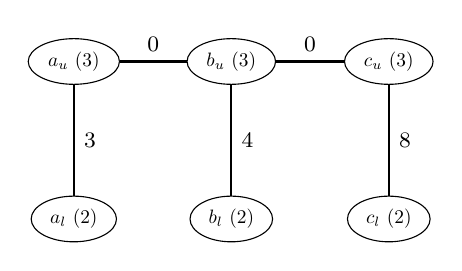
\begin{tikzpicture}
\usetikzlibrary{arrows}
\usetikzlibrary{shapes}
\usetikzlibrary{graphs}
\tikzstyle{every node}=[draw, ellipse, minimum size=10pt,align=center,scale=0.7]
\node at (0,2)(1){$a_{u}$ (3)};
\node at (2,2)(2){$b_{u}$ (3)};
\node at (4,2)(3){$c_{u}$ (3)};
\node at (0,0)(8){$a_{l}$ (2)};
\node at (2,0)(9){$b_{l}$ (2)};
\node at (4,0)(10){$c_{l}$ (2)};
%  \draw (1) -- (4) node [below]{8};

\path[every node/.style={font=\footnotesize},thick]
    (1) edge node[right] {3} (8)
    (2) edge node[right] {4} (9)
    (3) edge node[right] {8} (10)
    (1) edge node[above] {0} (2)
    (2) edge node[above] {0} (3);
\end{tikzpicture}
\caption*{Source: from author (2015).}\end{figure}

\begin{figure}[!h]
  \centering
  \caption{Substrate Graph resulted from transformation $\phi$.}\label{fig:transsub}
\begin{tikzpicture}
\usetikzlibrary{arrows}
\usetikzlibrary{shapes}
\usetikzlibrary{graphs}
\tikzstyle{every node}=[draw, ellipse, minimum size=10pt,align=center,scale=0.7]
\node at (0,3)(1){$A_{u}$ (3)};
\node at (2,3)(2){$B_{u}$ (3)};
\node at (4,3)(3){$C_{u}$ (3)};
\node [below=0.3cm of 3] at (1,2)(4){$U_{1}$ (1)};
\node [below=0.3cm of 3] at (3,2)(5){$U_{2}$ (1)};
\node [below=0.7cm of 4] at (1,1)(6){$L_{1}$ (1)};
\node [below=0.7cm of 4] at (3,1)(7){$L_{2}$ (1)};
\node [below=1cm of 7] at (0,0)(8){$A_{l}$ (2)};
\node [below=1cm of 7] at (2,0)(9){$B_{l}$ (2)};
\node [below=1cm of 7] at (4,0)(10){$C_{l}$ (2)};
%  \draw (1) -- (4) node [below]{8};

\path[every node/.style={font=\footnotesize},thick]
    (1) edge node[left] {8} (4) 
    (1) edge node[right] {8} (5)
    (2) edge node[left] {8} (4)
    (2) edge node[right] {8} (5)
    (3) edge node[left] {8} (4)
    (3) edge node[right] {8} (5)
    (4) edge node[right] {8} (6)
    (5) edge node[right] {8} (7)
    (8) edge node[right] {8} (6)
    (8) edge node[right] {8} (7)
    (9) edge node[left] {8} (6)
    (9) edge node[right] {8} (7)
    (10) edge node[left] {8} (6)
    (10) edge node[right] {8} (7);
\end{tikzpicture}
\caption*{Source: from author (2015).}\end{figure}

\begin{lemma} \label{lem:reduction}
  Any Bin Packing instance can be reduced to an instance of the Virtual Network Embedding Problem through procedure $\phi$.
\end{lemma}

\begin{proof}
There are~$n$ virtual nodes with demand three and~$n$ physical nodes with capacity three, therefore any feasible solution would map all virtual upper nodes to physical upper nodes. Likewise for physical and virtual nodes with capacity and demand two.
Hence, in the instance~$\phi(I)$ there is always a feasible mapping of the nodes.
Moreover, each of the~$n$ edges has to be mapped to a single path in the substrate graph between the upper nodes and the lower nodes.
Additionally, every path has to contain at least one edge between the middle nodes.
Those edges represent bins.
Mapping virtual links to those edges is tantamount to fit items in a bin.
%Hence, if a solution for $\phi(I)$ is given, a solution for $I$ can be obtained by selecting the first of the middle edges (the edges that link the middle nodes) in the $n$ paths.
%Moreover, if there is any feasible mapping for $\phi(I)$, the answer for the B\&P decision version is YES. 
%Therefore, if a polynomial algorithm exists that solves $\phi(I)$, we can use it to compute the answer to $I$ in polynomial time.
\end{proof}


\begin{lemma} \label{lem:transpol}
  The transformation $\phi(I)$ is polynomial in $|N|$.
\end{lemma}

\begin{proof}
The transformation $\phi$ creates two graphs, one with $2|N| + 2k$ nodes and $2|N|k + k$ edges and another with $2|N|$ nodes and $2n - 1$ edges. 
As $k < |N|$, and every item fits into a single bin, the size of the VNEP instance is limited polynomially by $|N|$, the number of items of $I$.
\end{proof}

\begin{lemma} \label{lem:polapp}
  If there exists a polynomial time algorithm that finds a feasible solution for $\phi(I)$, there is a polynomial time algorithm that finds a feasible solution for $I$.
\end{lemma}

\begin{proof}
All virtual nodes with demand three have to be mapped to substrate nodes with capacity three.
If one of the nodes of demand two is mapped to a substrate node of capacity three, there will be an unmapped virtual node of capacity three. 
Likewise, for nodes of capacity two.
%as there are only $|N|$ substrate nodes with capacity two, every one of the $|N|$ virtual nodes with demand two will be mapped to a substrate node of capacity two. 
Therefore there is always a feasible node mapping for $\phi(I)$. 
Note that the mapping order is not important: any virtual node with demand $x$ can be mapped to any physical node with capacity $x$.

If there is a feasible mapping for the virtual network of $\phi(I)$, the answer to I is YES:
Given a feasible mapping $M$, all virtual edges are mapped to a path in the substrate graph. 
Let $p_{i}$ be the path for which the virtual link~$i$, corresponding to the item~$i$, was mapped to. 
Let $j$ be the first substrate edge in $p_{i}$ that links the middle nodes. The edge~$j$ corresponds to the bin~$j$. Thus a solution for $I$ can be constructed if item~$i$ is allocated into bin~$j$. 
Since the capacity of all edges are not surpassed, the $k$~bins can hold the $|N|$~items.

If the answer for I is YES, there is a feasible mapping for $\phi(I)$:
Suppose that there is a configuration of the items into $k$ bins.
A solution for $\phi(I)$ can be constructed from a solution for $I$.
Suppose any feasible mapping $M$ of nodes for the virtual network (as it was shown before, there always exists a feasible mapping of nodes).
Let $f_{M}(u)$ be the substrate node for which the virtual node $u$ is mapped. 
Every virtual link $(u,v)$ corresponding to the item $i$ is mapped to the path $(f_{M}(u), x)$, $(x,y)$, $(y,f_{M}(v))$, where $(x,y)$ is the substrate edge corresponding to the bin $j$ for which the item $j$ was allocated in the solution for $I$.
Since the sum of the items in a bin $j$ does not exceed the capacity $B$, every virtual link can be mapped in the physical graph.
\end{proof}

\begin{lemma} \label{lem:cert}
  VNEP is an NP problem
\end{lemma}

\begin{proof}
  A solution for a VNEP instance I can be verified in polynomial time in the size of the instance. For every virtual node $u$ it suffices to check if the physical node $f_v(u)$ has enough capacity to host it, for every virtual link $(u,w)$ it suffices to check the path $p = f_e(u,w)$ is indeed a path (every adjacent edge shares one endpoint), and for every physical edge $e$, if all the links that are mapped in $e$ do not surpass its capacity.
\end{proof}

\begin{theorem} \label{th:npcomplete}
  VNEP is an NP-Complete problem.
\end{theorem}

\begin{proof}
The hardness of the VNEP problem follows from Lemmas~\ref{lem:reduction}-\ref{lem:cert}. 
\end{proof}

\begin{corollary} \label{co:nopoly}
  There is no polynomial time algorithm that finds a feasible solution for VNEP, unless $P=NP$.
\end{corollary}

\begin{proof}
  Suppose there is a polynomial time algorithm that finds a feasible solution (not necessarily optimal) for VNEP. From~\ref{lem:polapp}, it follow that there is a polynomial algorithm for solving BPP\@. 
  But this is only possible if $P = NP$.
\end{proof}

Corollary~\ref{co:nopoly} implies that there is probably no time efficient approximation algorithm for VNEP, since such an algorithm would provide a polynomial time algorithm to solve BPP.
